\chapter{Conclusions and Future Work}

% This chapter should summarize the whole project, it features and limitation. Moreover, you should give directions for future work

% In this space, before the first section, write an introductory paragraph for the chapter

We have introduced ASAR project as an software solution for digitizing the historical Arabic manuscript documents by using deep learning techniques. In this chapter, we let you catch a glimpse of how our journey looked like. We describe the challenges that we faced, the lessons that we learned, and summarize what we achieved. Finally, we discuss what the future may looks like.

\section{Faced Challenges}
% Mention all the problems/challenges that you faced while working with the project and how you overcome them
\subsection{Data Preparation}
Since we used VML-HD dataset that contains only annotated samples from 5 books with their XML files separately, the data wasn't ready for training.So, we firstly, cropped the all samples into word samples consist of 6,141 samples. Secondly, data cleaning is used to manually correct the mislabeled words and remove noisy words to become 5,429 samples. Finally, data augmentation is presented with different transformations to balancing the dataset and different patterns recognition.

\subsection{Resources}
Word spotting techniques didn't applied before in Arabic language that has open source projects. So, it was difficult to find any previous experiments on Arabic language. Also the practical resources was rare and not up to data, so we only depending on the mention scientific papers in the references section for understanding each module and how it works.

\subsection{Arabic Language Constrains}
In historical handwritten manuscripts, Arabic language faced difficult challenges weather in the word segmentation or character similarity. Segmentation for each line and word was difficult due to the connected components with each line to be segmented into words and characters. The similarity between Arabic characters was hard for the model to classify them correctly.

\subsection{Model Training}
The PHOSC model used in ASAR is a large complicated one that needs high resolution data of large amounts, and these constraints make it harder to train on the available resources we have. It needs a fast GPU of large memory size, preferably 16GB, which we didn't have and still be a problem. So, we used Standard\_NC6 compute on Azure cloud service, which consist of NVIDIA Tesla K80 GPU 24GB with 56GB RAM and 380GB disk storage.

\section{Gained Experience}
% Mentioned the experience/skills that you gained from working with the project

Working on developing \acrshort{asar} has been an enriching experience that we learned from in different ways:
\begin{itemize}[itemsep=1pt, topsep=5pt]
    \item Researching and reading dozens of papers to achieve working results helped us to be exposed to multiple methods in every sub module, and to see the evolution in the techniques through time.
    \item Working with different environments and integrate them together to build an intelligent system. Learning the process of end-to-end deep learning project linked with web and mobile application 
    \item We learned several tools and technologies, as described in the appendix A section, and learning to work on a remote server to train models on.
    \item Teamwork, effective collaboration, and asynchronous online communications.
\end{itemize}

\section{Conclusions}
% Write your conclusions regarding the project. Mention its features and limitations
Throughout this document, we demonstrated the idea of our project in order to analysis and digitizing the historical Arabic manuscript documents, and the steps applied when obtain an image following by preprocessing, line and word segmentation, and finally we recognizing it using PHOSC word spotting model. Also, we shown the results for each module and developed web and mobile applications to consume and integrate them together. 

\section{Future Work}
% Give possible extensions, enhancements and future work of you project, such that subsequent students could build on your work and develop larger systems/platforms.
ASAR has some limitations and multiple possible future extensions that would add value to the project. One of the limitations is limited Arabic corpus that we used into the training for word spotting (5,429 word) which will do better quality if there are much words, but this cost machine resource for training and manually collected. The feature that could be added is searching into the given manuscript document image for particular word by indexing each segmented word which could be a better search engine into the handwritten images. \\

Also, there are problems in ancient historical Arabic manuscripts for page segmentation cannot handle it using morphological preprocessing techniques. Fig \ref{fig:page-chanllenges} shows the challenges and the problems with page segmentation. The future work could be using Neural Networks or any related intelligent algorithms to address these problems:

\begin{itemize}[itemsep=1pt, topsep=5pt]
    \item Connected components for different Arabic words returning two or three words which cannot segmented a standalone word.
    \item Marginal notes which the segmentation cannot recognize it.
    \item The lines might be not straight. 
    \item Some manuscripts may contains a faded ink which the preprocessing techniques consider it as a noise and remove it.
\end{itemize}

\begin{figure}[!htb]
    \centering
    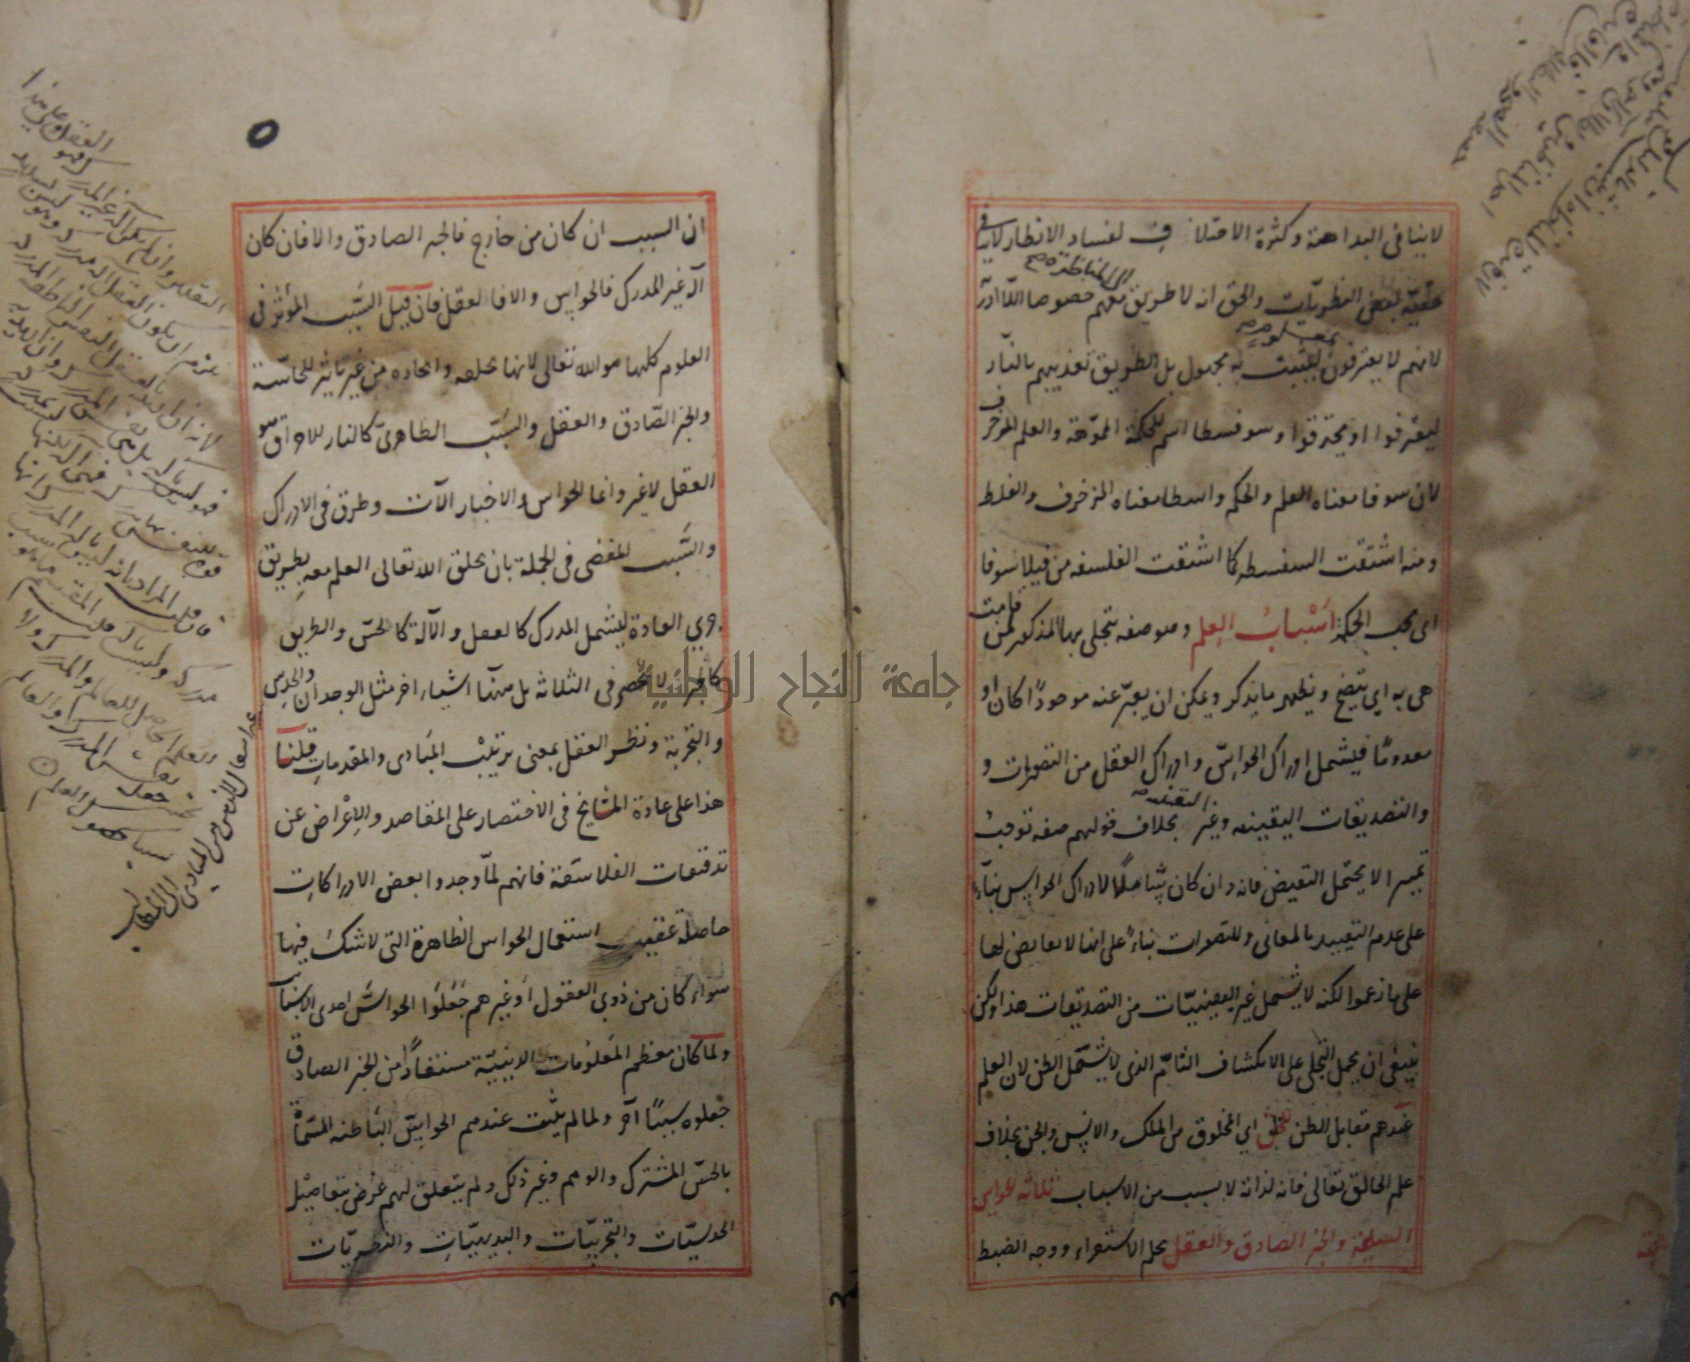
\includegraphics[width=10cm,height=7cm]{images/page-seg-challenges.png}
    \caption{Sample showing page segmentation challenges}
    \label{fig:page-chanllenges}
\end{figure}

\newpage

\addcontentsline{toc}{chapter}{Bibliography}
\printbibliography
